Section~\ref{sec:multidomain-SDN-deploy-and-config} describes the equipment,
Section~\ref{sec:multidomain-SDN-path-provisioning} describes control-plane
operations for path provisioning, and Section~\ref{sec:multidomain-SDN-FDT-access} describes the actions required
in the hosts at the ends of an L2 path to support our use case (dataset transfers).
Section~\ref{sec:multidomain-SDN-data-plane-expts} describes a simple experiment
to test data-plane connectivity across the dynamically configured inter-domain L2 VLAN paths.

\subsection{Equipment}
\label{sec:multidomain-SDN-deploy-and-config}

In a project called Dynamic Network System (DYNES) \cite{1742-6596-396-4-042065}, distributed instruments were deployed in 40 universities and 11 regional RENs. Our work
used the DYNES instruments in the following universities:
(i) U. Virginia (UVA), (ii) MAX GigaPoP (MAX), (iii) U. Wisconsin, Madison (UWisc), (iv) University of New Hampshire (UNH), (v) Internet2 Lab (I2Lab), (vi) Rutgers University,  (vii) Indiana University (IU), and (viii) Colorado University (CU). These university
networks are interconnected via their corresponding regional RENs, and Internet2 Advanced Layer 2 Service (AL2S) \cite{AL2S}. Fig.~\ref{fig:network} illustrates the setup using just two university domains as an example.
\begin{figure}
\centering               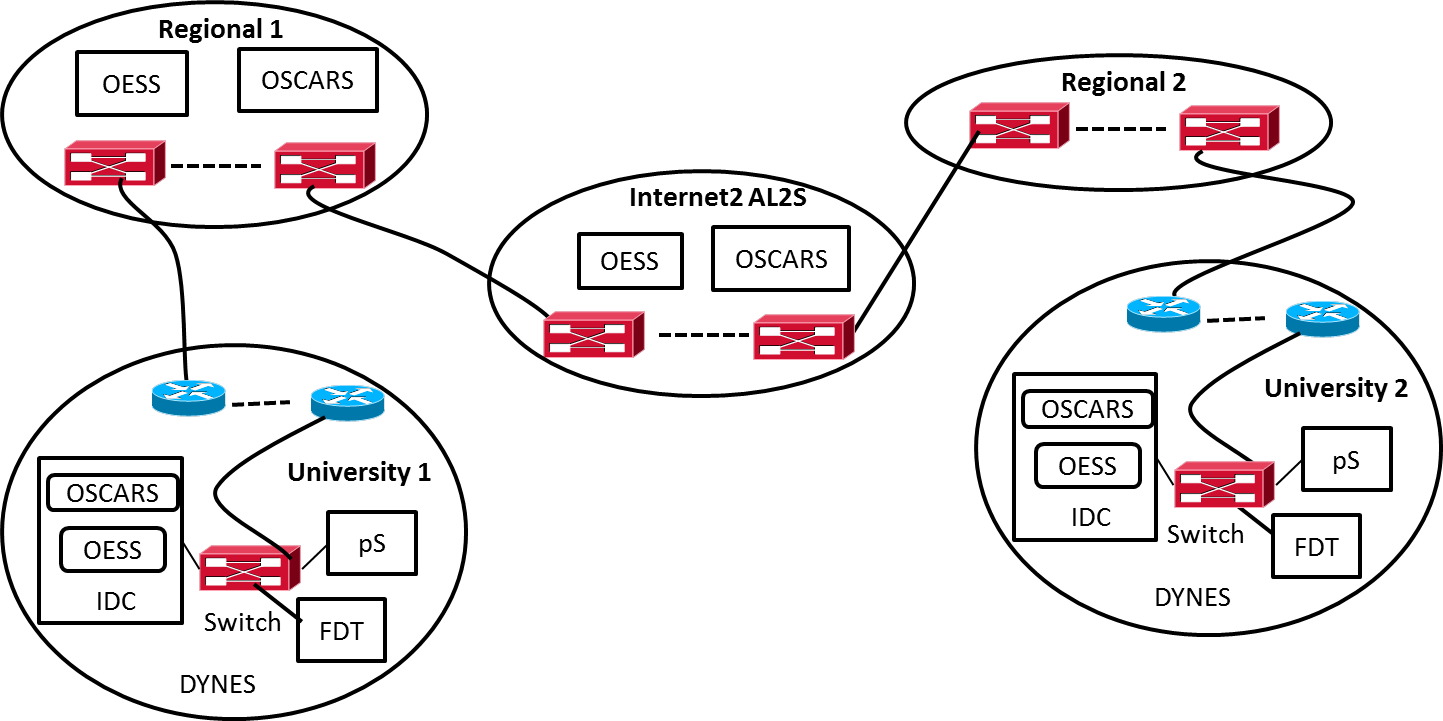
\includegraphics[width=0.7\textwidth]{figures/multi-domain-network.png}
\caption{An illustration of our multi-domain dynamic L2 path service deployment; Fast Data Transfer (FDT) server; Inter-Domain Controller (IDC); perfSONAR (pS) host; Open Exchange Software Suite (OESS); On-Demand Secure Circuits and Advance Reservation System (OSCARS); Advanced Layer 2 Service (AL2S)}
\label{fig:network}
\end{figure}

Each university
campus DYNES equipment, as shown in Fig.~\ref{fig:network},
consists of three hosts: Fast Data Transfer (FDT) server, Inter-Domain Controller (IDC) host, perfSONAR (pS) \cite{perfSONAR} host,
and one Ethernet switch (which is OpenFlow enabled in some sites). The FDT server runs data-transfer applications, the IDC host runs the control-plane software (OSCARS, and OESS at sites with an OpenFlow-enabled switch), and the pS host runs active-measurement tools for monitoring network performance.

Some regional RENs such as Regional 1 in Fig.~\ref{fig:network}
run OSCARS and OESS controllers to offer dynamic
L2 path service while others such as Regional 2 in
Fig.~\ref{fig:network} offer only static L2 path service and
hence do not deploy OESS and OSCARS.
As can be expected with the roll-out of a new networking
service, organizations will slowly deploy the service
one-at-a-time. Static L2 path service is available from most RENs
and university campus networks, and can be used to bridge gaps in the
dynamic L2 service offering.

Internet2's Advanced Layer-2 Service (AL2S) network has 39 OpenFlow-enabled
Ethernet switches, as shown in Fig~\ref{fig:AL2S}, and is operated in L2 Virtual LAN (VLAN) mode.
AL2S delivers a strategic advantage for leaders in research and education (R$\&$E) by providing effective and efficient wide area 100 gigabit Ethernet technology. AL2S allows users to create their own VLANs on the Internet2 AL2S backbone. Static or Dynamic, point-to-point or multipoint, intra-domain or inter-domain, AL2S puts control of the backbone VLANs into the users' hands for the creation of purpose-built private circuits using infrastructure already in place. AL2S is available to 279 higher education institutions include Univeristy of Virginia. AL2S uses OESS for controlling the OpenFlow switches, and OSCARS for inter-domain L2 paths.
\begin{figure*}[htbp!]
\centering 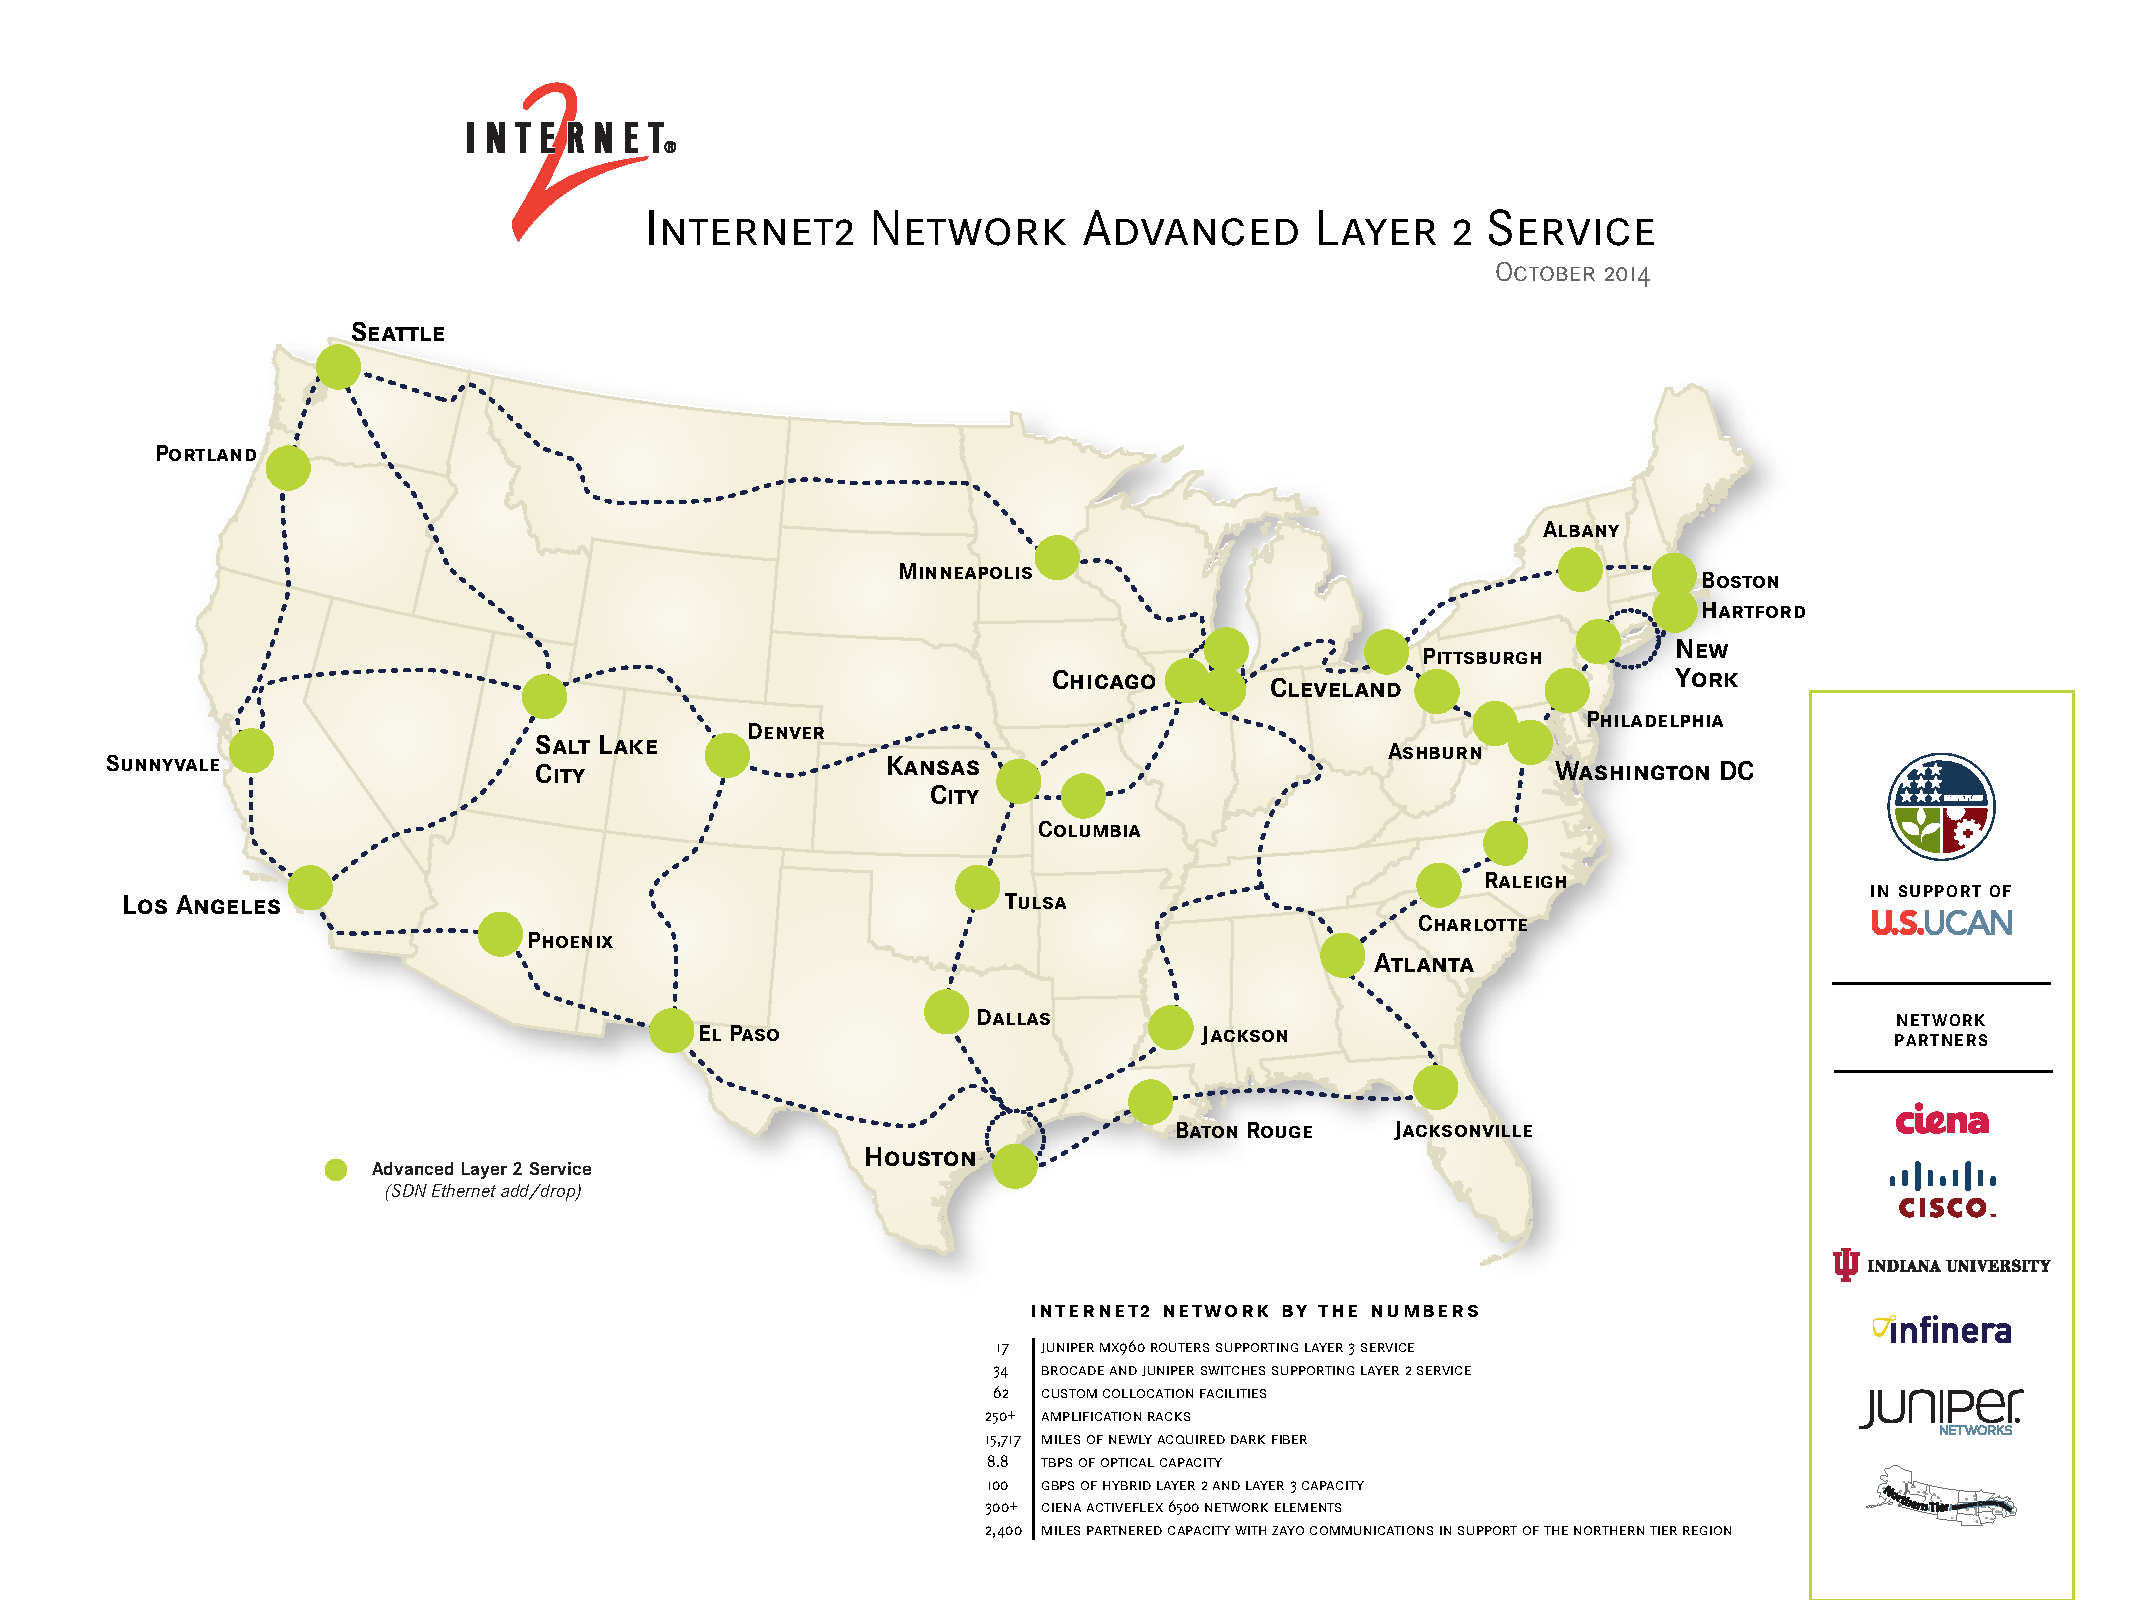
\includegraphics[width=0.80\textwidth]{figures/AL2S.pdf}
\caption{Internet2 Advanced Layer 2 Service (AL2S) Network}
\label{fig:AL2S}
\end{figure*}

We \emph{first} describe how the
DYNES equipment was configured at each site.
\emph{Next}, we describe the actions needed within campuses between the
location of the DYNES equipment and the campus edge. \emph{Finally},
we describe the actions required from regional RENs
that did not deploy this dynamic L2 path service.

\textbf{Step 1.} At each DYNES site, we logged in to the OpenFlow
enabled switch, configured the IP address of the IDC host
on which the OESS (OpenFlow controller) is being run, and
added the set of ports to be controlled by the OESS into
the switch's OpenFlow instance (only one instance is used).
The OpenFlow switch models used by the DYNES project
support \emph{hybrid-switch} mode in which OpenFlow controlled
and traditionally configured ports can co-exist on the switch.
However, these switches do not support \emph{hybrid-port} mode in
which each individual port can be controlled by both the
OpenFlow controller and traditional configuration methods.

The next set of operations at each DYNES site consisted of
(i) initiating OESS and OSCARS on the IDC host, (ii) providing the OESS with the switch's control-port IP address,
and (iii) configuring OESS and OSCARS through their Web
UIs. Specifically, the OESS UI is used to set the remote-link
information for the data-plane port of the peering network.
For example, the UVA DYNES switch port 1 is connected
to say port 1 of a UVA campus router. A static VLAN was
configured from port 1 of this UVA campus router through
the other UVA campus routers, and through the regional
REN (MARIA) routers to the MARIA router port that is
connected to port et-3/0/0.0 on the Internet2 AL2S switch
in Ashburn, VA. This static VLAN serves as the remote
link between UVA DYNES network and Internet2 AL2S.
Information about this remote link is entered into the UVA
DYNES OESS to identify the peering domain, node, and
port. The counterpart action was performed at Internet2's
OESS for the UVA DYNES switch remote link. This remote-link information was provided manually to Internet2. The
OESS UI is also used to configure the set of allowed VLANs
on each port of the DYNES switch.

UVA DYNES OSCARS needed to be configured with a server certificate, and the certificate owner and issuer information needed to be manually communicated to Internet2's administrator for configuration of Internet2's AL2S OSCARS. These certificates are used in the authentication
process for inter-domain L2 path requests.

\textbf{Step 2.} Most of the involved campus networks and regional
RENs support static L2 path services. This allowed us to request and obtain provisioned L2 paths with a specified set of
VLAN IDs from campus network administrators. These L2
paths cut across the campus switches/routers between the
DYNES equipment and the campus edge router. Having the
capability to establish static L2 paths allows for a gradual
introduction of OpenFlow switches under OESS control into
campus networks.

\textbf{Step 3.} Similarly, we contacted regional REN administrators to obtain static L2 paths with specified VLAN IDs
across their networks to Internet2. Again this capability of using static L2 paths allows for a gradual addition of
dynamic L2 path service by different regionals at different
times, and yet support dynamically created end-to-end L2
paths.

The above experience shows the various steps required to
configure OSCARS and OESS in each organization that is
ready to support dynamic L2 service, as well as the feasibility of using static L2 paths through networks whose organizations are not as-yet ready for the dynamic service.

\subsection{Path/VLAN provisioning through switches}
\label{sec:multidomain-SDN-path-provisioning}

This section describes the process of establishing a new VLAN via the OESS UI \cite{OESS}. We use the term ``path'' if the VLAN has just two
endpoints, and the term ``multipoint VLAN'' if there are multiple endpoints.

After user authentication in the OESS UI through the login process, the OSCARS IDC workgroup should
be selected. Then in the Actions tab, the user should select the \texttt{Create a New VLAN} option. The system then guides the user through a 6-step procedure to provision a VLAN.

\paragraph{Step 1:  Basic characteristics}
Fig.~\ref{fig:oessbasic} shows a screenshot of the first step for a local circuit, and Fig.~\ref{fig:oessbasic-interdomain} shows a screenshot of the first step for an inter-domain circuit.
In both cases, the user should enter a human-readable name for the VLAN being created in the
\texttt{Description} field. For inter-domain paths, the user is offered the option of specifying
bandwidth for the circuit (see Fig.~\ref{fig:oessbasic-interdomain}), but not for intra-domain (local) paths (see Fig.~\ref{fig:oessbasic}).
 If the user wants a failed VLAN that had been automatically routed to a backup path to be restored to the primary path, the \texttt{Restore to Primary} field should be enabled. If the VLAN can stay routed on the backup path, this field can left in the \texttt{Off} state. The \texttt{Multipoint Static MAC Routing} field allows a user to associate a destination MAC addresses with each endpoint of a multipoint VLAN. Packets destined to such a configured MAC address will be forwarded to only the corresponding endpoint rather than to all endpoints as would happen if this feature was left disabled, or for packets with destination MAC addresses that were not attached to any endpoints of the multipoint VLAN.
 This field is only offered for local (intra-domain) paths (see Fig.~\ref{fig:oessbasic}), and
 not for inter-domain paths (see Fig.~\ref{fig:oessbasic-interdomain}). The \texttt{Type of Circuit} field should be set by the user to \texttt{Local}, if the VLAN traverses the single domain controlled by the particular OESS whose UI is being accessed. If the VLAN will
need to traverse multiple domains, the user should select the \texttt{Interdomain} option. This
option will cause the OESS to obtain all accessible endpoints from the
OSCARS topology service as described in Section~\ref{sec:OESS}, and load these into the UI in the next step for endpoint selection.

\begin{figure}[htb!]
\centering
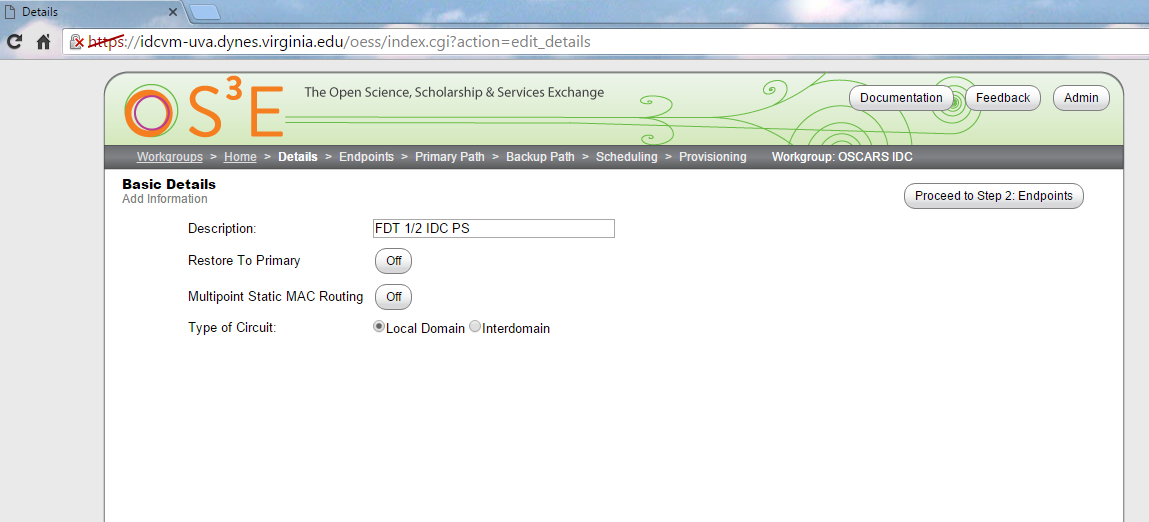
\includegraphics[width=0.8\textwidth]{figures/oess-basic.png}
\caption{OESS UI Step 1: Choose basic characteristics for an intra-domain path}
\label{fig:oessbasic}
\end{figure}

\begin{figure}[htb!]
\centering
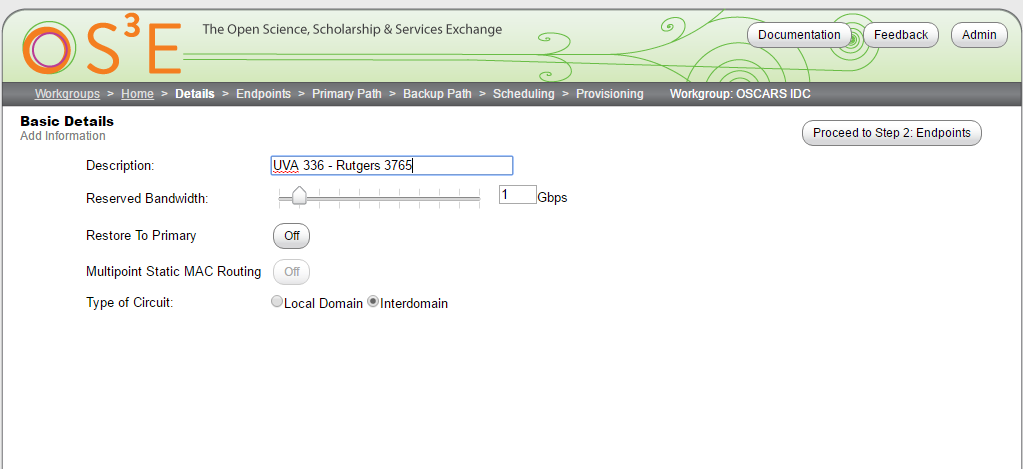
\includegraphics[width=0.8\textwidth]{figures/oess-basic2.png}
\caption{OESS UI Step 1: Choose basic characteristics for an inter-domain path}
\label{fig:oessbasic-interdomain}
\end{figure}



\paragraph{Step 2: Endpoints and VLAN IDs}
Fig.~\ref{fig:oesspoints} shows Step 2, in which the user selects the endpoints of the VLAN.
For each endpoint, the user needs to provide a corresponding VLAN ID. The user starts by clicking on the dot in the map displayed on the screen. In this example, the single dot represents the UVA DYNES switch. Since the \texttt{Type of Circuit} field was set to \texttt{Local} in Step 1,
OESS displays just the seven endpoints of the UVA DYNES network (on the bottom right corner). Specifically, these endpoints are ports on the single UVA DYNES switch served by the OESS being used for this provisioning process. When the user clicks on a port that should be an endpoint in the VLAN, OESS displays a window in which the user is required to provide a specific VLAN ID. Each workgroup is provided rights to use specific VLAN IDs for each endpoint. Hence
authorization is run by OESS allows before a particular VLAN ID is used for provisioning. In this
example, the user has selected four interfaces, specifically ports 0/19, 0/24, 0/22, and 0/20,
of the UVA DYNE switch,
and hence these interfaces are displayed under \texttt{Endpoints} in the main part of the screen.
The user has selected the same VLAN ID 332 for all four endpoints.
\begin{figure}[htb!]
\centering
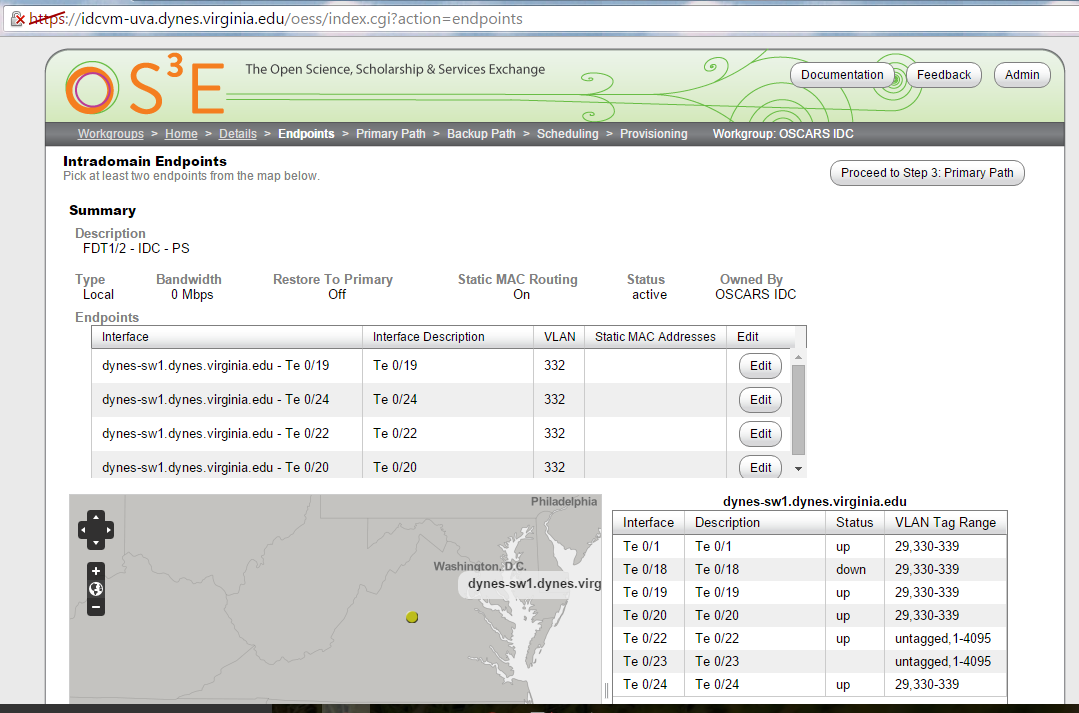
\includegraphics[width=0.8\textwidth]{figures/oess-points.png}
\caption{OESS UI Step 2: Selection of endpoints and VLAN IDs}
\label{fig:oesspoints}
\end{figure}

\paragraph{Step 3: Select primary path}
Fig.~\ref{fig:oessprimary} shows the OESS UI screenshot for Step 3 in which the user can select a path or ask OESS to suggest the shortest path. If a user is not particular about the selected path, users can click on the\texttt{ Suggest Shortest Path} button, and OESS will find the shortest path between the selected endpoints. Alternatively, a users can click on links to add or remove them from a path. The path must connect the endpoints and must not have any loops. For the example show, since the three interfaces are on the same UVA DYNES switch, there is only one possible multipoint VLAN.
\begin{figure}[htb!]
\centering
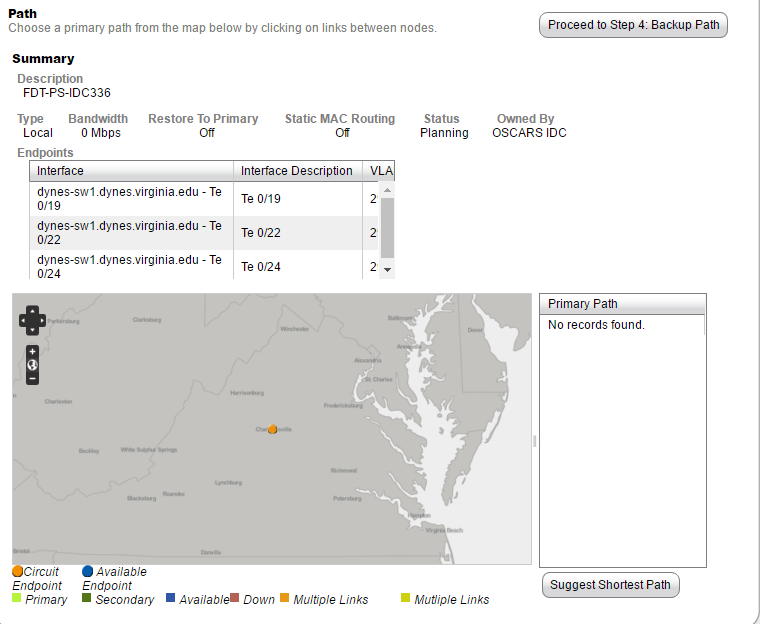
\includegraphics[width=0.8\textwidth]{figures/oess-primary.png}
\caption{OESS UI Step 3: Primary path selection}
\label{fig:oessprimary}
\end{figure}

\textbf{Step 4: Select backup path}
In Step 4, a user can select a backup path for automatic switch-over from the primary path in case of
failures. If the user clicks on the \texttt{Suggest Shortest Path} button, the OESS will attempt to find an path that has minimal overlap with the primary path.  Selection of a backup path is optional. Fig.~\ref{fig:oessbackup} shows a screenshot of the OESS UI Step 4.
\begin{figure}[htb!]
\centering
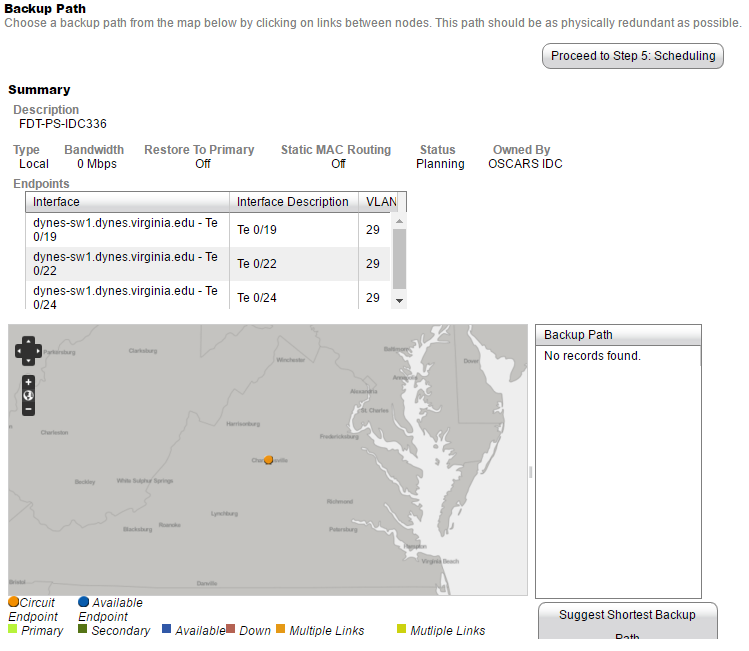
\includegraphics[width=0.8\textwidth]{figures/oess-backup.png}
\caption{OESS UI Step 4: Backup path selection}
\label{fig:oessbackup}
\end{figure}

\textbf{Step 5: Scheduling}
\begin{figure}[htb!]
\centering
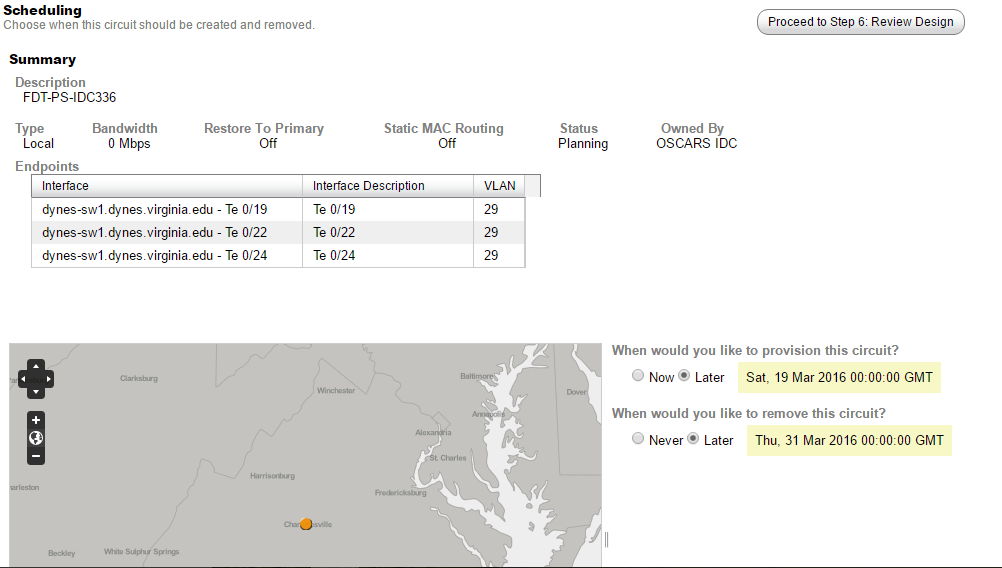
\includegraphics[width=0.8\textwidth]{figures/oess-schedule.png}
\caption{OESS UI Step 5: Circuit scheduling}
\label{fig:oessschedule}
\end{figure}
Fig.~\ref{fig:oessschedule} shows a screenshot of the OESS UI Step 5, in which a user can specify
a start time and release time for the circuit. In the example shown, the user
has requested a later
start time (not ``now''), and has specified a particular future date when the circuit should be released.

\paragraph{Step 6: Review design and submit circuit request}
Users are given an opportunity to review the design before selecting
the \texttt{Submit Circuit Request}.
Fig.~\ref{fig:oessreview} shows the corresponding OESS UI screenshot.
\begin{figure}[htb!]
\centering
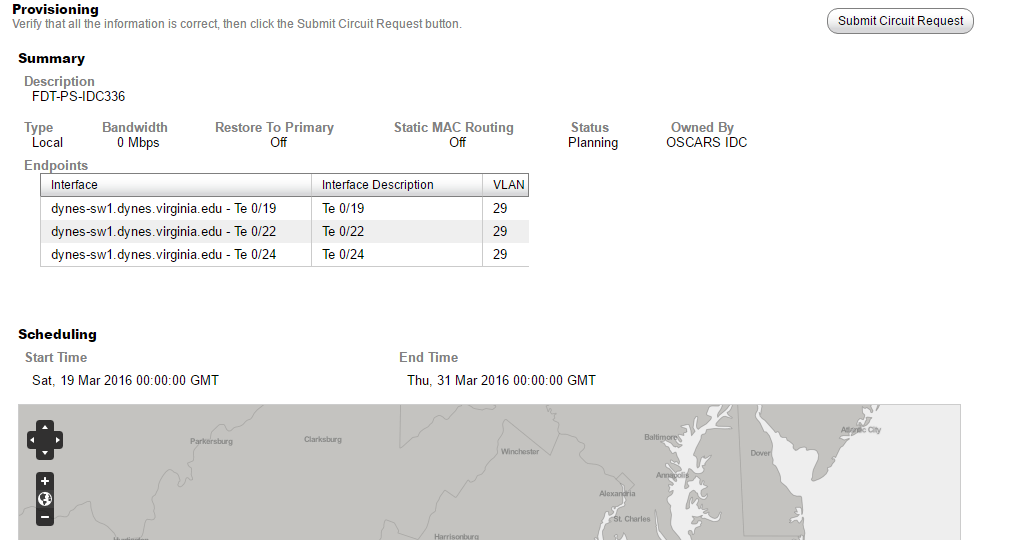
\includegraphics[width=0.8\textwidth]{figures/oess-review.png}
\caption{OESS UI Step 6: Review design}
\label{fig:oessreview}
\end{figure}

If the OESS is successful in setting up the circuit between the selected endpoints
at the specified rate, in the time interval specified in Step 4, a success message
is displayed to the user through the UI. If not, a failure message is displayed.
One of the drawbacks of the current software is that failure messages do
not offer a cause for the failure.

\subsection{Path Configuration at Hosts}
\label{sec:multidomain-SDN-FDT-access}
Three steps are required to configure the FDT hosts at the
ends of an L2 path: (i) a VLAN with the appropriate VLAN
ID is configured on the FDT NIC that is connected to the
DYNES switch, (ii) IP addresses on the same subnet are
assigned to the VLANs configured at the two FDT hosts,
and (iii) the traffic control (\texttt{tc}) Linux utility is configured
to rate limit outgoing traffic to the L2-path rate used in the
path-reservation phase.
\begin{figure}
\centering
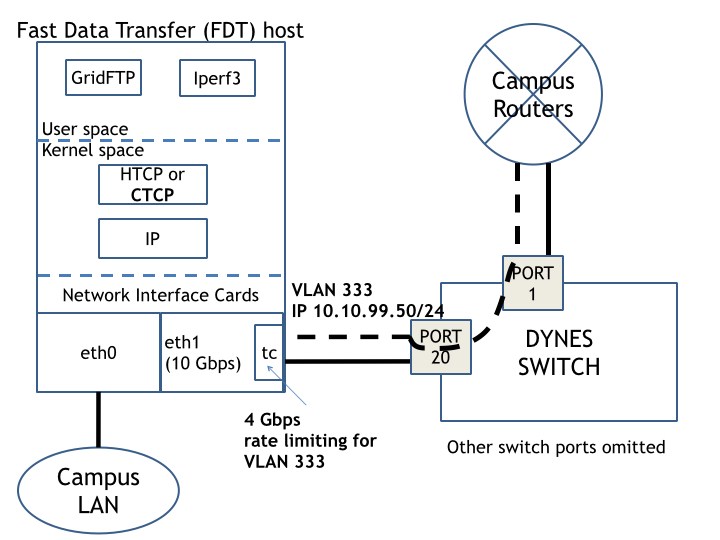
\includegraphics[width=0.6\textwidth]{figures/uvadynes.png}
\caption{Configuring the Fast Data Transfer (FDT) host for the L2 path}
\label{fig:uvadynes}
\end{figure}

Fig.~\ref{fig:uvadynes} illustrates the UVA DYNES data-plane with a configured VLAN for the end-to-end L2 path to the IU FDT.
However before discussing the details of Fig.~\ref{fig:uvadynes}, recall the example end-to-end L2 path described in Fig.~\ref{fig:AL2S} between
port 19 of the DYNES switch in the University 1 network,
and port 20 of the DYNES switch in the University 2 network of Fig.~\ref{fig:AL2S}. While the endpoints specified in the request
to the OESS are the two switch ports, the L2 path essentially
extends between the FDTs at University 1 and University 2
as the specified switch ports are connected to the FDTs.

Therefore, the VLAN ID used on the interface from the FDT
to the DYNES switch in the request to the OESS needs to
now be configured in the FDT. In the example shown in
Fig.~\ref{fig:uvadynes}, the VLAN ID used in the request to the OESS for
port 20 of the UVA DYNES switch for the L2 path to the
IU FDT was 333. Now, using the Linux \texttt{vconfig} command
in the UVA FDT, the user or application needs to configure
VLAN 333 on the \texttt{eth1} NIC, which is the one connected to
port 20 of the DYNES switch.

The second step that needs to be executed on the FDT is a
configuration of an IP address associated with the newly created VLAN. For this purpose the Linux \texttt{ifconfig} command
is used. Fig.~\ref{fig:uvadynes}shows that private IP address 10.10.99.50
is assigned to VLAN 333 on \texttt{eth1}. IP packets sent out
with source IP address equal to 10.10.99.50 will be carried
in tagged Ethernet frame headers with VLAN ID set to 333.

Fig.~\ref{fig:uvadynes} also shows that the FDT host has another NIC, \texttt{eth0}
for connectivity to the campus LAN. This interface for logging into the FDT remotely using an ssh client.

The reason for needing to configure IP on the VLAN is to allow for the usage of existing applications, such as GridFTP
and \texttt{nuttcp}, and transport-layer protocols such as HTCP \cite{HTCP}
as illustrated inside the FDT in Fig.~\ref{fig:uvadynes}. Packets sent on the
end-to-end L2 path are not subject to L3 (IP) header based
packet forwarding because all switches on the path have
been provisioned to execute packet forwarding based on the
VLAN ID. IP headers are nevertheless included/extracted at
the FDT servers because of the applications' use of TCP/IP
sockets.

Furthermore, the private IP addresses configured for the
FDT VLANs at the two ends need to belong to the same
subnet to avoid having to add destination-specific routes to
the IP-routing table in the FDTs. For this L2 path, the
VLAN ID used on the port of the IU DYNES switch was
2399 and the IP address assigned to VLAN 2399 on the
Ethernet NIC in the IU FDT host was 10.10.99.40.

In our usage of these L2 paths,
we manually executed these VLAN and IP address configuration commands at the FDT hosts, having procured privileged access for the execution of these commands. However, for general-purpose use of L2 path-based networking, applications should be integrated (through shell scripts or with
modifications) with a signaling-client module that issues requests for paths to OESS, handles responses, and additionally configures VLANs and IP addresses at the FDTs. Further, an end-to-end session protocol is required to exchange
subnet identifier/mask information to ensure that the private IP addresses assigned to the VLANs at the two end
FDTs match. Since the FDT and IDC servers have multiple Ethernet interfaces, one of which is connected to the campus IP-routed
infrastructure, e.g., \texttt{eth0} in the FDT shown in Fig.~\ref{fig:uvadynes}, L3 IP
service is used for all signaling messages.

Finally, Fig.~\ref{fig:uvadynes} shows that the Linux \texttt{tc} utility is used in the
FDT host to limit the rate at which the 10Gbps \texttt{eth1} NIC
transmits frames. The example VLAN shown was created
with a 3 Gbps rate request; therefore, \texttt{tc} would have been
configured to rate limit VLAN-333 Ethernet frames to 3
Gbps.

\subsection{Data plane Experiments}
\label{sec:multidomain-SDN-data-plane-expts}

This section describes the methodology used to test a newly provisioned VLAN.
It not only verifies that the VLAN has been successfully provisioned across the network(s), 
but also verifies the configuration actions at the end hosts.
\begin{figure}[htb!]
\centering
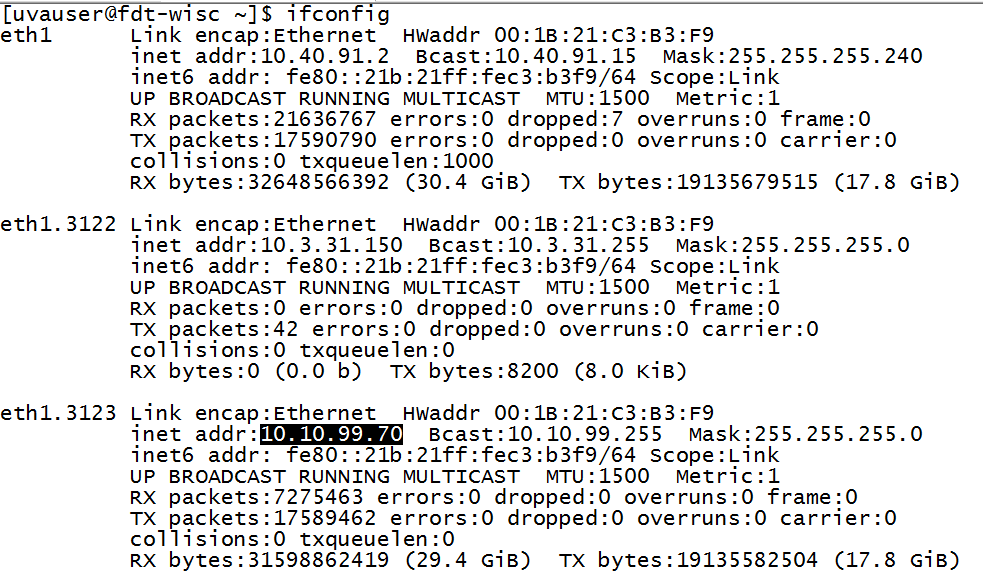
\includegraphics[width=0.8\textwidth]{figures/ifconfig.png}
\caption{Linux utility \texttt{ifconfig}}
\label{fig:ifconfig}
\end{figure}
An interdomain circuit was configured from the FDT at UWisc to the FDT at UVA. The VLAN ID
at the UWisc FDT was 3123, and at the UVA FDT, it was 336. The IP addresses/subnet masks 10.10.99.70/24 and 10.10.99.50/24 were assigned to the UWisc FDT VLAN and UVA FDT VLAN,
respectively.

Before running an end-to-end data-plane test, the Linux utility \texttt{ifconfig} was used to check the configuration of the VLANs at both ends. Fig.~\ref{fig:ifconfig} shows the UWisc interface \texttt{eth1} was configured with a VLAN with ID 3123, and this VLAN was
 assigned IP address 10.10.99.70 with subnet mask /24.

Next, the \texttt{ping} command was executed to test the reachability across this newly configured VLAN path from UWisc FDT to UVA FDT.
 Fig.~\ref{fig:ping} shows that the UVA FDT VLAN was reachable from the UWisc FDT,
 as the latter receives a reply to the ping command sent to IP address 10.10.99.50, which is
 the address that was assigned to VLAN 336 at the UVA FDT interface. Success of this
\texttt{ping} execution verifies that the L2 path was successfully setup across all five domains,
UWisc, CIC OmniPoP (regional REN for UWisc), Internet2 AL2S, MARIA (regional REN for UVA),
and UVA. Further it attests to the successful configuration of the two end hosts.

\begin{figure}[htb!]
\centering
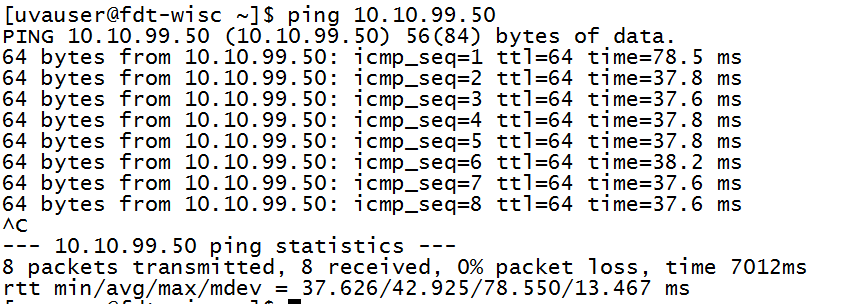
\includegraphics[width=0.8\textwidth]{figures/ping.png}
\caption{Linux utility ping}
\label{fig:ping}
\end{figure}

